\documentclass{prologArticle}
\usepackage{float}
\usepackage{enumitem}
\usepackage{tabularx}
\usetikzlibrary{babel} % used to make edge possible


% use \declare{test/} to create a new variable nam\space
% you can use the root namespace too if you want to
% use \setvalue and \getvalue to manipulate data
\setvalue{meta/title =miniprojet - WhalEscape}
% Uncomment the line below to disable small caps in the section titles
\setvalue{formatting/section = \large\raggedright}

% If you want to use your own lststyle:
%\setvalue{formatting/listings/default = yourlststyle}

% \lstset{language=Java}
\newcolumntype{b}{X}
\newcolumntype{s}{>{\hsize=.3\hsize}X}
\newcolumntype{d}{>{\hsize=.8\hsize}X}

\begin{document}

\buildtitle



\section{Introduction}
Le but de ce projet était d'appliquer en pratique ce qui a été vu en cours durant le semestre. Pour cela il a fallu penser au dévelopement en prenant compte tout ce qui a été vu. Le temps imparti ne nous permettait pas de dévelloper tout les éléments d'un jeu-vidéo au maximum. Toutefois nous nous sommes efforcés de ne négliger aucun aspect général du jeu.

\section{Story}

\begin{figure}[H]
    \centering
    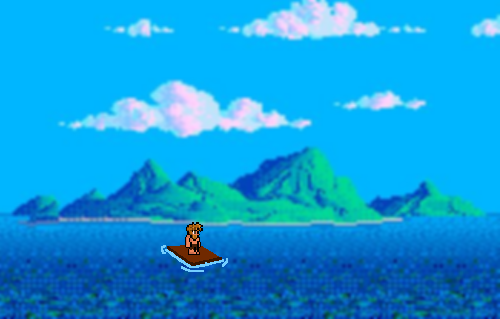
\includegraphics[width=0.6\textwidth]{res/story1.png}
    \caption{Jonah sur son radeau}
\end{figure}

\begin{figure}[H]
    \centering
    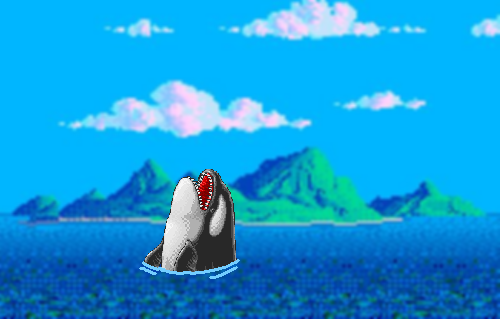
\includegraphics[width=0.6\textwidth]{res/story2.png}
    \caption{La baleine mange Jonah et son embarquation}
\end{figure}

Jonah a été victime d'un naufrage sur une île déserte. Seul survivant, il parvient a fabriquer un radeau et à quitter l'île. En s'éloignant de l'île, une baleine l'a attaqué et l'a avaler avec une partie de son radeau. Le joueur doit maintenant contrôller Jonah et l'aider à s'échapper de la baleine, en commençant dans les intestins. Il pourra utiliser les objets qu'il trouvera. Ces objets proviennent des restes du radeau ou ont été avalé par la baleine auparavant. Il devra aussi faire face à des ennemis tel que des blobs de sucs gastriques ou les restes d'autres naufragés malchanceux. Il devra remonter le système digestif de l'animal en passant par les intestins et l'estomac avant d'atteindre l'évent qui lui permettera de sortir.

\begin{figure}[H]
    \centering
    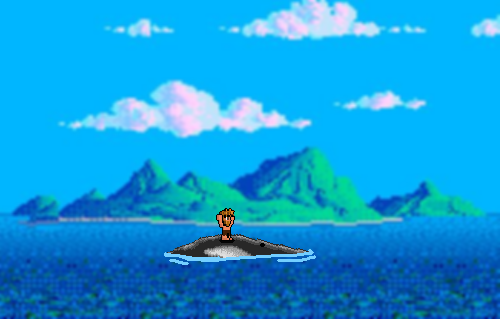
\includegraphics[width=0.6\textwidth]{res/story3.png}
    \caption{Jonah a réussi à sortir de la baleine}
\end{figure}

\subsection{Protagonist}

Le joueur se met dans la peau de Jonah un naufragé qui s'est fait gober par une baleine.

Verbes d'actions:
\begin{enumerate}
    \item déplacement gauche droite
    \item sauter
    \item attaquer si équipé d'une rame
\end{enumerate}

\subsection{Antagonists}

\subsubsection{Blobs}
Des bulle d'acide flottent à traver le niveau de l'estomac. Elles ont pour buts de géner le joueur dans sa progression et de le faire tomber dans l'acide.

Verbes d'actions:
\begin{enumerate}
    \item Déplacement sinuosoidale gauche droite dans l'air
    \item Pousser Jonah
\end{enumerate}

\subsubsection{Squelette}
Les squelette d'anciennes victimes de la baleine veillent à ce qu'aucun intrus se balade dans le corps de la baleine. Ils patrouillent dans les intestins.

Verbes d'actions:
\begin{enumerate}
    \item Patrouille à pied de gauche à droite
    \item Attaquer si un ennemi se trouve devant lui.
\end{enumerate}

\subsubsection{Baleine}
Elle vous a gobé mais elle ne vas pas s'arrêter là, son corps est un véritable labyrinthe et plein de pieges.

Aucun verbe d'actions
\newpage
\section{Mechanics}

\subsection{Rules}

\subsubsection{Générales}
\begin{itemize}
    \item Si Jonah tombe dans le vide il meurt
    \item Jonah a 2 points de vie
    \item À chaque fois qu'il se fait taper par un enemi, il perd un point de vie
    \item Lorsque Jonah n'a plus de points de vie il meurt
    \item Jonah peut attaquer seulement si il est équipé d'une rame
    \item Pour s'équiper de rame, il doit marcher dessus
    \item Au bout de 3 coups porté avec la rame, celle-ci échappe des mains de Jonah et il doit la ramasser à nouveau
    \item Lorsque Jonah meurt, il recommence au début du niveau
\end{itemize}

\subsubsection{Level 1}
\begin{itemize}
    \item Jonah doit trouver la zone qui le fera sortir de ce niveau
    \item Les enemis sont des squelettes d'autres naufragés malchanceux.
\end{itemize}

\begin{figure}[H]
    \centering
    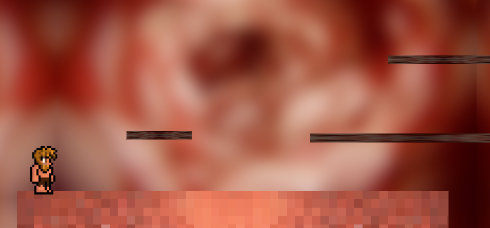
\includegraphics[width=0.8\textwidth]{res/level1.png}
    \caption{Départ du niveau 1}
\end{figure}

\subsubsection{Level 2}

\begin{itemize}
    \item Jonah doit monter les plateformes rapidement pour éviter de se faire rattraper par l'acide de l'estomac
    \item Si Jonah se fait toucher par l'acide (rattrapé par la caméra) il meurt
    \item Des blobs d'acides vont traverser l'écran afin de gêner Jonah dans sa progression
    \item La caméra monte indépendamment du personnage. Si le joueur touche le bord inférieur de la caméra, il meurt.
\end{itemize}

\begin{figure}[H]
    \centering
    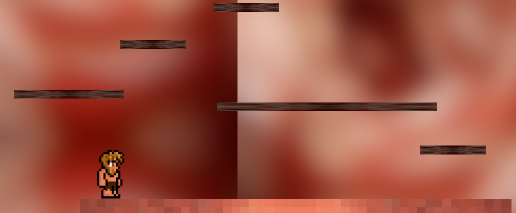
\includegraphics[width=0.8\textwidth]{res/level2.png}
    \caption{Départ du niveau 2}
\end{figure}


\section{Aesthetics}

\subsection{Aspect visuel}
Nous avons décidé de ne pas tout réaliser en vrai pixel art comme nous avions initialement prévu. En effet, tout dessiner nous même aurait pris beaucoup trop de temps. Pour beaucoup d'élément nous avons simplement pixelisé des photos existantes ou nous avons cherché des sprite sheets gratuites sur internet.

L'idée était de donner au maximum au joueur l'impression d'être dans un corps vivant sans trop le dégouter. Il a fallu flouter les photos d'estomacs que nous avions pour ne pas heurter la sensibilité de certain.

\subsubsection{Jonah}
Pour Jonah nous nous sommes fortement inspiré de l'image de Robinson Crusoé que les gens ont en tête. Nous avons utilisé le rig des personnages de Terraria comment template de base et nous avons redessiné Jonah par dessus.

\begin{figure}[H]
    \centering
    
\includegraphics[width=\textwidth]{res/jona_sheet.png}
    \caption{Les frames d'animation de Jonah}
\end{figure}

\subsubsection{Blob}
L'idée avec le blob était de faire quelque chose de semblable à l'idée que l'on peut se faire des acides présent dans un estomac tout en restant simple pour pouvoir le dessiner facilement. La couleur verte a été choisie pour bien mettre en valeur que c'est un élément avec lequel on interagit dans le jeu.

\begin{figure}[H]
    \centering
    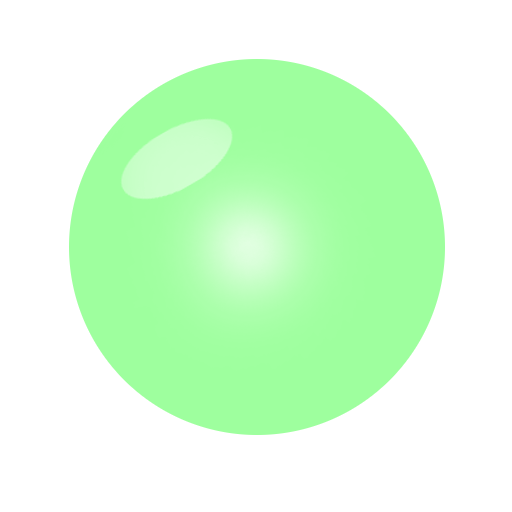
\includegraphics[width=0.1\textwidth]{res/blobb.png}
    \caption{L'illustration utilisé pour notre blobb}
\end{figure}

\subsubsection{Squelette}
Les squelettes vivant dans notre baleine sont les restes des naufragés qui ont été précédemment avalés par la baleine. En raison du manque de temps, nous avons utilisé une sprite sheet gratuite trouvée sur internet pour l'animation et l'affichage des squelettes.

\begin{figure}[H]
    \centering
    
\includegraphics[width=0.1\textwidth]{res/Skeleton.png}
    \caption{L'illustration utilisé pour les squelettes}
\end{figure}

\subsubsection{La rame}

La rame est le seul objet que Jonah peut ramasser et utiliser. On a réaliser un icône ainsi qu'une série de sprites où Jonah attaque équipé de la rame.

\begin{figure}[H]
    \centering
    
\includegraphics[width=0.1\textwidth]{res/rame.png}
    \caption{Icône utilisé pour la rame}
\end{figure}

\begin{figure}[H]
    \centering
    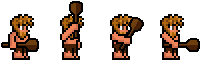
\includegraphics[width=0.3\textwidth]{res/jonaharmed.png}
    \caption{Jonah qui attaque avec la rame}
\end{figure}

\subsubsection{La baleine}

Le sprite de la baleine vient du jeux Metal Slug. Là encore nous avons utilisé un sprite existant car nous n'avons pas eu le temps de dessiner nous même un sprite.

\subsubsection{Fins de niveaux}

Pour le premier niveau, la fin est symboliser par un trou qui permet à Jonah de passer des instestins à l'estomac tandis que la fin du second niveau est visuellement représenté par l'évent qui permettera à Jonah de sortir de la baleine.

\begin{figure}[H]
    \centering
    
\includegraphics[width=0.1\textwidth]{res/ovent.png}
    \caption{L'évent qui permet de s'échapper}
\end{figure}

\begin{figure}[H]
    \centering
    
\includegraphics[width=0.1\textwidth]{res/door.png}
    \caption{Le trou qui permet de rentrer dans l'estomac}
\end{figure}

\subsection{Aspect sonore}
Nous avons voulu donner le maximum de retour à l'utilisateur que nous pouvions. C'est pour cela que nous avions mis un son pour beaucoup d'élément. Tout nos éléments à part le thème du jeu sont issues du site internet "freesound"

\subsubsection{Jonah}
\begin{enumerate}
    \item Son lorsqu'il saute
    \item Son lorsqu'il frappe avec la rame
    \item Son lorsqu'il se fait toucher
\end{enumerate}

\subsubsection{Blob}
Le blob est plus a considéré comme une plateforme en mouvement qu'un personnage en termes d'actions. C'est pour ça que nous n'avons pas jugé approprié de lui mettre un son.

\subsubsection{Squelette}
\begin{enumerate}
    \item Son lorsqu'il frappe
    \item Son lorsqu'il se fait toucher
\end{enumerate}

\subsubsection{Thème}
Pour la musique de thème nous avons utilisé un remix 8bit de la chanson thème de Pirates of the Carribean que l'on a trouvé libre de droits sur youtube.


\section{Technology}
Tout le jeu est fait avec Unity3D, avec C\# comme language de programmation. Nous avons aussi utilisé Aseprite, un éditeur de pixel art, et Gimp pour réaliser les éléments visuels du jeu. Pour le versionning du code et la collaboration, nous avons utilisé Git et Github.


\section{Conclusion}
Nous avons pris beaucoup de plaisir à faire ce projet. Nous avons pu explorer plus en détail des mécaniques d'Unity et explorer la multi-disciplanirité qu'est le dévellopement de jeu-vidéo. Ceci nous a permis de nous rendre compte des multiples casquettes qu'un développeur de jeux vidéo doit endosser lorsqu'il travaille au sein d'une équipe réduite. Nous aurions aimé pouvoir consacrer plus de temps au projet pour pouvoir vraiment fignoler notre jeux et ajouter un troisième niveau.

\end{document}
